\title{Développement}
\subtitle{}
\author{}
\institute{}
\date{}
\begin{frame}
	\maketitle
\end{frame}

\begin{frame}
	\frametitle{Développement}
	\framesubtitle{Séparation vue-modèle}
	\textbf{Avantages}
	\begin{itemize}
		\item Débogage
		\item Modularité
		\begin{itemize}
			\item Séparation des threads
			\item Travail en équipe
		\end{itemize}
	\end{itemize}

	\textbf{Inconvéniants}
	\begin{itemize}
		\item Vite limitant
		\item Difficile à maintenir
	\end{itemize}
\end{frame}

\begin{frame}
	\frametitle{Développement}
	\framesubtitle{Multithreading}

	\textbf{Pourquoi ?}
	\begin{itemize}
		\item Algorithmes longs
		\item Généricité IA-Joueur
		\item Consommation d'énergie équivalente (GIL)
	\end{itemize}
	\textbf{Comment ?}
	\begin{itemize}
		\item Machines à état
		\item Ownership pattern
	\end{itemize}
\end{frame}

\begin{frame}
	\frametitle{Développement}
	\framesubtitle{Intelligence artificielle}

	\begin{itemize}
		\item Orienté Objet
		\item Une seule méthode à surcharger
		\item Pas à se soucier des threads ou des règles
	\end{itemize}

	\begin{figure}[b]
		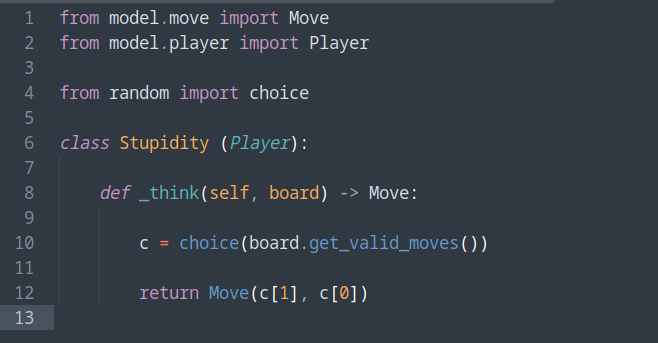
\includegraphics[width=0.5\textwidth]{img/stupidity.png}
		\caption{Code intégral de l'IA "stupidity"}
	\end{figure}
\end{frame}

\begin{frame}
	\frametitle{Développement}
	\framesubtitle{Base de données}

	\begin{figure}
		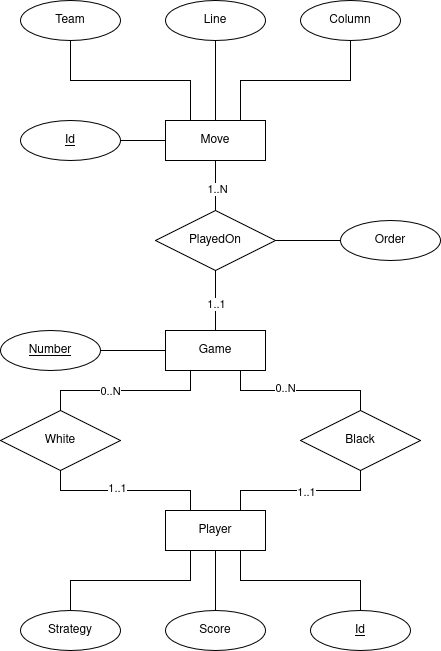
\includegraphics[width=0.2\textwidth]{img/entity_relationship.png}
		\caption{Modèle entité-relation de notre base de données}
	\end{figure}
\end{frame}

\begin{frame}
	\frametitle{Développement}
	\framesubtitle{Base de données}
	\begin{figure}
		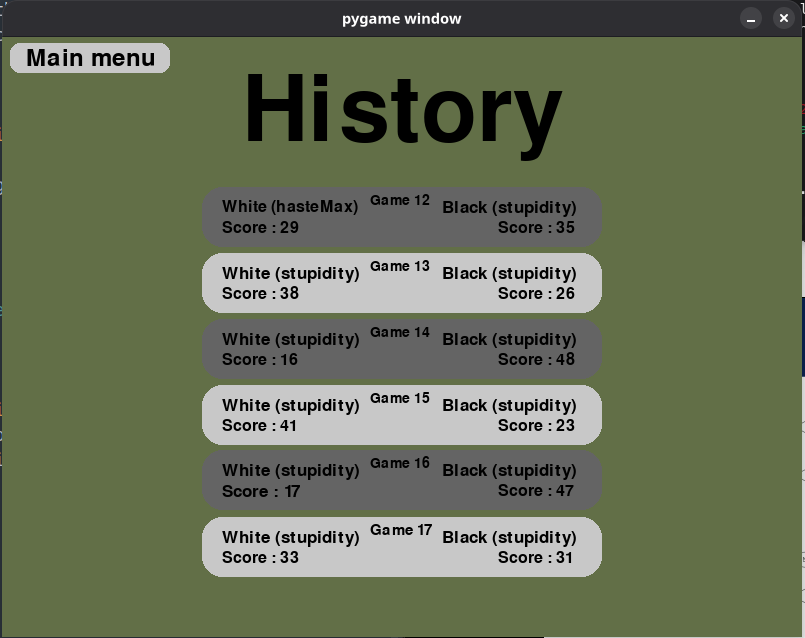
\includegraphics[width=0.5\textwidth]{img/history.png}
		\caption{Affichage dans l'application}
	\end{figure}
\end{frame}

\begin{frame}
	\frametitle{Développement}
	\framesubtitle{Interface utilisateur}

	\begin{itemize}
		\item Abre de \lstinline{Widget}
		\item Algèbre linéaire
		\item Similaire au HTML/CSS
	\end{itemize}
\end{frame}

\begin{frame}
	\frametitle{Développement}
	\framesubtitle{Interface utilisateur}
	\centering

	\begin{math}
	\begin{pmatrix}
		scale_x & 0       & position_x \\
		0       & scale_y & position_y \\
		0       & 0       & 1
	\end{pmatrix}
	\end{math}
\end{frame}

\begin{frame}
	\frametitle{Développement}
	\framesubtitle{Interface utilisateur}
	\centering

	\textbf{Exemple avec un widget $B$ enfant d'un widget $A$:}
	\vfill

	\begin{math}
	\begin{pmatrix}
		scale_Ax & 0       & position_Ax \\
		0       & scale_Ay & position_Ay \\
		0       & 0       & 1
	\end{pmatrix}
	\times
	\begin{pmatrix}
		scale_Bx & 0       & position_Bx \\
		0       & scale_By & position_By \\
		0       & 0       & 1
	\end{pmatrix}
	\end{math}
\end{frame}

\begin{frame}
	\frametitle{Développement}
	\framesubtitle{Interface utilisateur}
	\centering
	\textbf{Exemple avec un widget $B$ enfant d'un widget $A$:}
	\vfill

	\begin{math}
	=
	\begin{pmatrix}
		scale_Ax \cdot scale_Bx & 0 & scale_Ax \cdot position_Bx + position_Ax \\
		0       & scale_Ay \cdot scale_By & scale_Ay \cdot position_By + position_Ay \\
		0       & 0       & 1
	\end{pmatrix}
	\end{math}
\end{frame}

\begin{frame}
	\frametitle{Développement}
	\framesubtitle{Interface utilisateur}
	\begin{figure}
		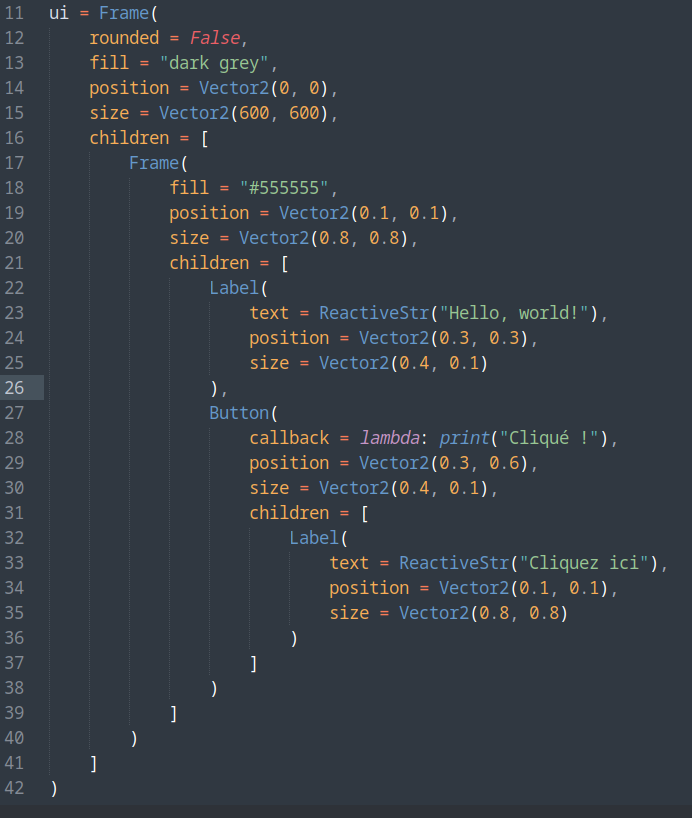
\includegraphics[width=0.3\textwidth]{img/code_ui.png}
		\caption{Code d'une UI}
	\end{figure}
\end{frame}
\begin{frame}
	\frametitle{Développement}
	\framesubtitle{Interface utilisateur}
	\begin{figure}
		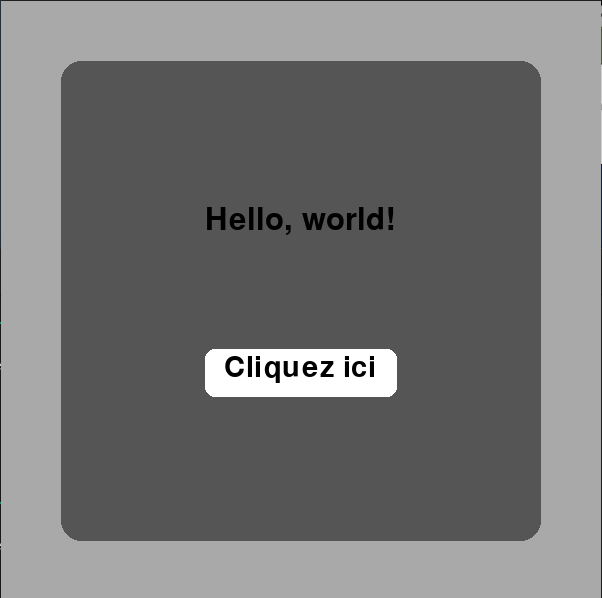
\includegraphics[width=0.3\textwidth]{img/ui.png}
		\caption{Résultat d'une UI}
	\end{figure}

\end{frame}